%This work is licensed under the Creative Commons License Attribution 4.0 International (CC-BY 4.0)
%https://creativecommons.org/licenses/by/4.0/legalcode
\documentclass[rgb]{standalone}
\usepackage{tkz-euclide}
\definecolor{myorange}{hsb}{0.0833, 1, 0.8}
\definecolor{mygreen}{hsb}{0.3333, 1, 0.8}
\definecolor{myblue}{hsb}{0.5833, 1, 0.8}
\definecolor{mymagenta}{hsb}{0.8333, 1, 0.8}
\begin{document}
	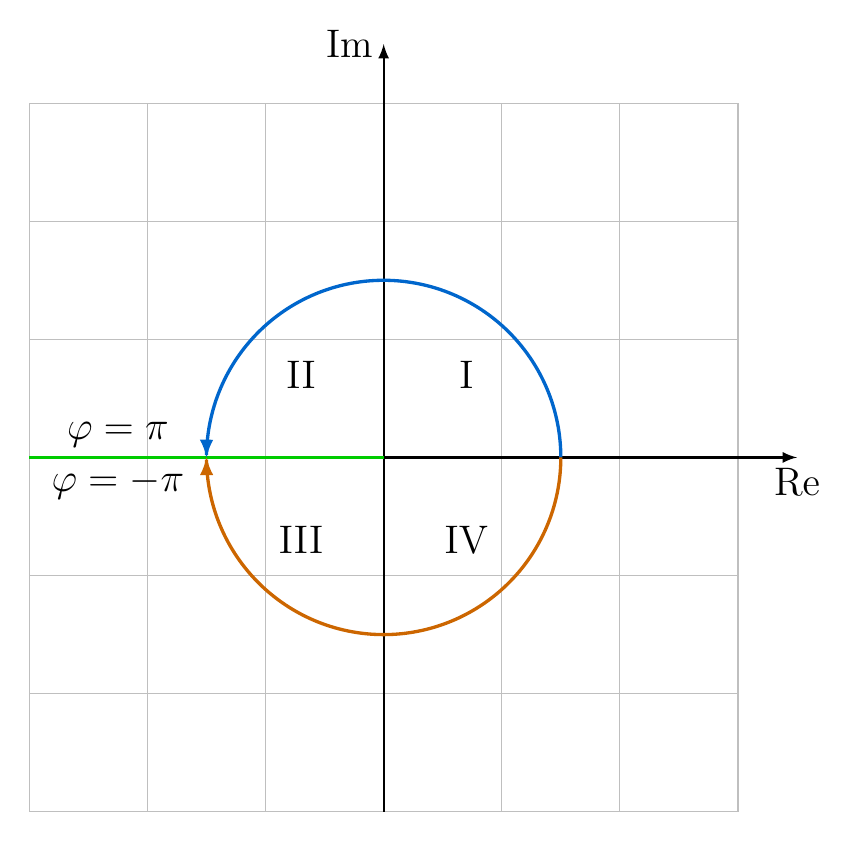
\begin{tikzpicture}[scale=1.5, font=\Large]
		% Coordinate system
		\tkzInit[xmin=-3,xmax=3,ymin=-3,ymax=3]
		\tkzGrid[color=lightgray]
		\tkzDrawX[thick,label=Re]
		\tkzDrawY[thick,label=Im]
		\draw[very thick, mygreen] (0,0) -- (-3,0);
		\draw[very thick,domain=0:180, myblue, smooth, samples=200, variable=\x,-latex] plot ({1.5*cos(\x)}, {1.5*sin(\x)});
		\draw[very thick,domain=0:-180, myorange, smooth, samples=200, variable=\x,-latex] plot ({1.5*cos(\x)}, {1.5*sin(\x)});
		% Labels
		\node[anchor=center] at (0.7,0.7){I};
		\node[anchor=center] at (-0.7,0.7){II};
		\node[anchor=center] at (-0.7,-0.7){III};
		\node[anchor=center] at (0.7,-0.7){IV};
		\node[above] at (-2.25,0){$\varphi=\pi$};
		\node[below] at (-2.25,0){$\varphi=-\pi$};
	\end{tikzpicture}	
\end{document}